\chapter{الموازنات الترموديناميكية والأنظمة المفتوحة}\label{ch:b2:open-systems}

تناول ترموديناميك مجلد السنة الأولى الأنظمة المغلقة ---
أي كتلة ثابتة من غاز في أسطوانة، تُضغط وتُسخَّن وتتمدد. لكن
الآلات التي تدفئ بيوتنا فعلًا، وتبرّد طعامنا، وتصنع
كهرباءنا يعبرها \emph{جريان}: فالبخار ينساب عبر
عنفة محطة توليد بمئات الكيلوغرامات في الثانية، والمبرِّد
يدور عبر الضاغط والمكثِّف والصمام والمبخِّر في مضخة حرارية،
والهواء يجري عبر الضاغط وغرفة الاحتراق في محرك نفاث. وكل مكوّن
\emph{\omterm{def:b2:open-systems:cv}{نظام مفتوح}}، أي منطقة من الفضاء تدخلها المادة وتخرج
منها، ويجب إعادة كتابة المبدأين الأول والثاني له. وإعادة الكتابة قصيرة
--- والمفتاح أن المائع المدفوع إلى النظام يحمل، زيادةً على
طاقته الداخلية، العمل المبذول في دفعه، ولهذا يكون
\emph{\omterm{thm:b2:open-systems:firstlaw}{الإنتالبي}}، لا الطاقة الداخلية، طاقةَ الجريان الطبيعية.
وهذا الفصل يقيم موازنات الكتلة والطاقة والإنتروبيا للأنظمة
المفتوحة في \omterm{def:b2:open-systems:cv}{الجريان المستقر}، ويطبّقها على الأجهزة الابتدائية ---
\omterm{prop:b2:open-systems:devices}{المنفث}، \omterm{prop:b2:open-systems:devices}{والخانق}، والضاغط، والعنفة، \omterm{prop:b2:open-systems:devices}{والمبادل الحراري} --- ويركّب
تلك الأجهزة في الدورتين اللتين تقيسهما مسألة نهاية الأسبوع: مضخة
حرارية ومحطة توليد بخارية.

\begin{omfigure}
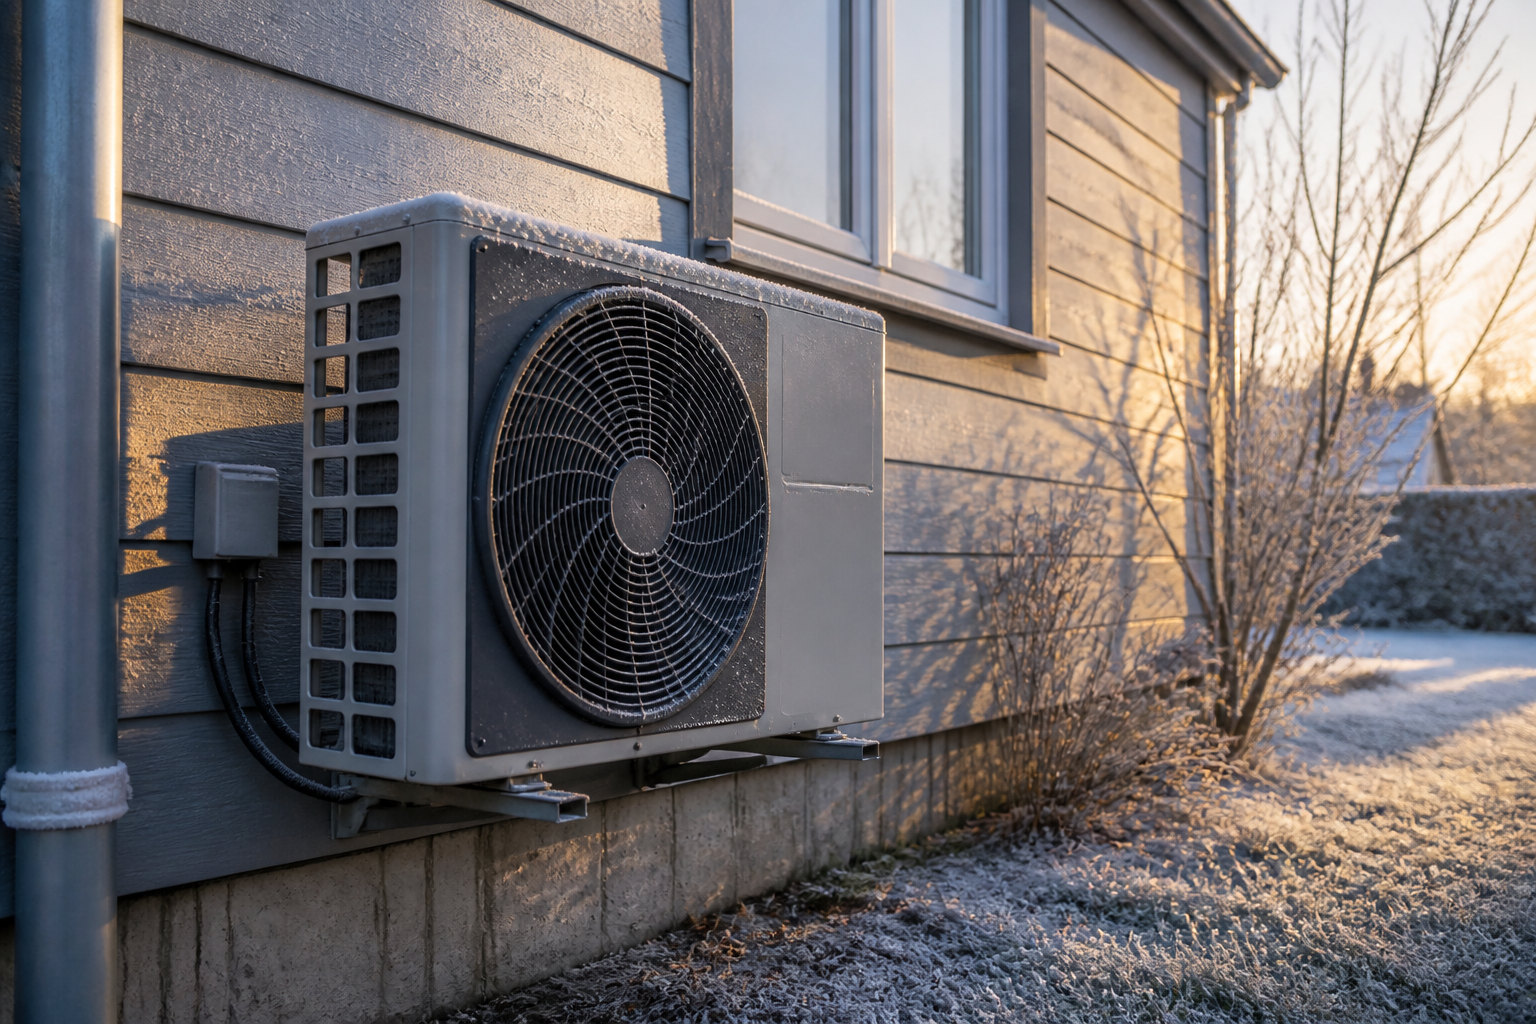
\includegraphics[width=0.58\linewidth]{images/book4/ai/b4-27-heat-pump-winter.png}

{\small الوحدة الخارجية لمضخة حرارية في صباح شتوي: مروحة
تسحب الهواء البارد على المبخِّر، وفي الداخل ضاغط،
ومكثِّف، وصمام تنقل تلك الحرارة، مضاعفةً ثلاث مرات أو أربعًا،
إلى البيت.}
\end{omfigure}

\section{الأنظمة المفتوحة وموازنة الكتلة}

\begin{definition}[النظام المفتوح، وحجم التحكم، والجريان المستقر]\label{def:b2:open-systems:cv}
\emph{النظام المفتوح}\index{نظام مفتوح} منطقة ثابتة من الفضاء،
هي \emph{حجم التحكم}\index{حجم التحكم} $\Sigma$، يحدّها
سطح يدخل المائع عبره ويخرج (أي مقطعا الدخول والخروج)
ويمكن أن تُتبادَل عبره الحرارة والعمل مع
الخارج؛ والعمل المتلقَّى عبر أجزاء متحركة (عمود، أو مكبس)
غير الجريان نفسه هو \emph{العمل النافع}\index{عمل نافع}
$W_{\text{u}}$ (أي عمل العمود). والجريان \emph{مستقر}\index{جريان
مستقر} حين يكون كل حقل داخل $\Sigma$ مستقلًّا عن الزمن: فتكون الكتلة
والطاقة والإنتروبيا المحتواة في $\Sigma$ ثابتة.
\end{definition}

\begin{proposition}[موازنة الكتلة]\label{prop:b2:open-systems:mass}
عبر مقطع مساحته $S$ يتحرك فيه المائع الذي كثافته $\rho$
بالسرعة الوسطى $c$ عموديًّا عليه يجري \emph{التدفق
الكتلي}\index{تدفق كتلي} $\dot m = \rho c S$ (بالوحدة \unit{kg/s}). وفي
\omterm{def:b2:open-systems:cv}{الجريان المستقر} يخرج ما يدخل: $\sum_{\text{دخول}}\dot m = \sum_{\text{خروج}}
\dot m$؛ ومن أجل تيار واحد يكون $\dot m$ نفسه عند الدخول والخروج،
$\rho_1c_1S_1 = \rho_2c_2S_2$ --- وهي \omterm{thm:b2:fluid-kinematics:continuity}{معادلة الاستمرار} في
\cref{ch:b2:fluid-kinematics} مكاملةً على المقطع.
\end{proposition}

\begin{proof}
الكتلة في $\Sigma$ ثابتة، فتتوازن التدفقات.
\end{proof}

\section{المبدأ الأول من أجل نظام مفتوح}

\begin{theorem}[الموازنة الطاقية لجريان مستقر أحادي التيار]\label{thm:b2:open-systems:firstlaw}
من أجل \omterm{def:b2:open-systems:cv}{جريان مستقر} تدفقه الكتلي $\dot m$ يدخل في الحالة 1
ويخرج في الحالة 2، متلقيًا الاستطاعة النافعة (استطاعة العمود)
$P_{\text{u}}$ والاستطاعة الحرارية $P_{\text{حراري}}$،
\[
\dot m\,\Big[(h_2 - h_1) + \tfrac12(c_2^2 - c_1^2) + g(z_2 - z_1)\Big]
= P_{\text{u}} + P_{\text{حراري}} ,
\]
أو، في وحدة كتلة المائع العابر النظام،
\[
\Delta h + \Delta\big(\tfrac12c^2\big) + g\,\Delta z = w_{\text{u}} + q .
\]
و\emph{الإنتالبي}\index{إنتالبي (في جريان)} $h = u + Pv$ يحلّ محلّ
الطاقة الداخلية: والمقدار $Pv$ هو \emph{عمل الجريان}، أي العمل الذي يبذله
المائع الأعلى ليدفع وحدة كتلة إلى الداخل، ناقصًا ما يُبذَل لدفعها
إلى الخارج.
\end{theorem}

\begin{proof}
اتبع النظام المغلق المؤلف من المائع داخل $\Sigma$ عند $t$ زائدًا
الكتلة $\dd m = \dot m\,\dd t$ التي توشك أن تدخل؛ وعند $t + \dd t$ يكون
مؤلفًا من المائع داخل $\Sigma$ (بالحالة نفسها، فهو \omterm{def:b2:open-systems:cv}{مستقر}) زائدًا
الكتلة $\dd m$ التي خرجت. وقد تغيرت طاقته بمقدار
$\dd m\,[(u_2 + \tfrac12c_2^2 + gz_2) - (u_1 + \tfrac12c_1^2 + gz_1)]$. وقد
تلقّى $P_{\text{u}}\dd t + P_{\text{حراري}}\dd t$، زائدًا عمل
قوى الضغط عند الدخول، $P_1S_1 \times c_1\dd t = P_1v_1\,\dd m$
(دفعًا للكتلة إلى الداخل)، ناقصًا ما عند الخروج، $P_2v_2\,\dd m$. والمبدأ
الأول من أجل هذا النظام المغلق، مع $u + Pv = h$، يعطي النتيجة.
\end{proof}

\begin{omfigure}
\begin{tikzpicture}[scale=0.95, >=stealth]
  \draw[thick, rounded corners=6pt, fill=omDef!8] (1.2,0) rectangle (6.2,2.6);
  \node[font=\scriptsize] at (3.7,1.9) {حجم التحكم $\Sigma$ (مستقر)};
  % أنبوب الدخول
  \draw[thick] (-0.6,0.5) -- (1.2,0.5); \draw[thick] (-0.6,1.1) -- (1.2,1.1);
  \fill[omExo!40] (-0.5,0.52) rectangle (0.1,1.08);
  \node[font=\scriptsize, above] at (-0.2,1.12) {$\dd m$};
  \draw[->, omExo, thick] (-1.4,0.8) -- (-0.6,0.8);
  \node[font=\scriptsize, left] at (-1.4,0.8) {$\dot m$, $h_1$, $c_1$, $z_1$};
  % أنبوب الخروج
  \draw[thick] (6.2,1.5) -- (8.0,1.5); \draw[thick] (6.2,2.1) -- (8.0,2.1);
  \fill[omExo!40] (7.3,1.52) rectangle (7.9,2.08);
  \node[font=\scriptsize, above] at (7.6,2.12) {$\dd m$};
  \draw[->, omExo, thick] (8.0,1.8) -- (8.8,1.8);
  \node[font=\scriptsize, right] at (8.8,1.8) {$h_2$, $c_2$, $z_2$};
  % العمود
  \draw[->, omThm, very thick] (3.7,-0.8) -- (3.7,0) node[pos=0, below, font=\scriptsize] {$P_{\text{u}}$ (العمود)};
  \draw[->, omThm, very thick] (5.5,3.4) -- (5.5,2.6) node[pos=0, above, font=\scriptsize] {$P_{\text{حراري}}$};
  % دفعا الضغط
  \node[font=\scriptsize, omExo] at (0.3,0.2) {$P_1v_1$ يدفع داخلًا};
  \node[font=\scriptsize, omExo] at (7.2,1.2) {$P_2v_2$ يدفع خارجًا};
\end{tikzpicture}

{\small \omterm{def:b2:open-systems:cv}{النظام المفتوح} \omterm{def:b2:open-systems:cv}{المستقر}: النظام المغلق المتبوع خلال $\dd
t$ هو محتوى $\Sigma$ زائدًا الكتلة الداخلة، ثم المحتوى
زائدًا الكتلة الخارجة؛ وعمل الضغط عند المقطعين يحوّل $u$
إلى $h = u + Pv$.}
\end{omfigure}

\begin{remark}[استعمال المبدأ الأول]\label{rem:b2:open-systems:using}
من أجل غاز مثالي $\Delta h = c_p\Delta T$؛ ومن أجل سائل $\Delta h \approx
c\,\Delta T + v\,\Delta P$ (والحدّ الثاني هو عمل المضخة)؛ ومن أجل بخار
يُقرأ $h$ من جداول أو مخططات. والحدّ الحركي مهمَل عادةً:
فعند \qty{10}{m/s}، $c^2/2 = \qty{50}{J/kg}$، في وجه
\qty{1}{kJ/kg} لكل كلفن من الهواء --- ولا يهمّ إلا في \omterm{prop:b2:open-systems:devices}{المنافث} و
ريش العنفات، حيث تبلغ السرعات مئات الأمتار في الثانية. وأما الحدّ
الكموني، $g\Delta z \approx \qty{10}{J/kg}$ في المتر، فيهمّ في
ماء السدّ، ولا يهمّ قط في دورة غازية. ومع عدة مداخل ومخارج
تُقرأ الموازنة $\sum_{\text{خروج}}\dot m\,h - \sum_{\text{دخول}}\dot m\,h =
P_{\text{u}} + P_{\text{حراري}}$ (بإهمال الحدّين الحركي والكموني).
\end{remark}

\section{المبدأ الثاني من أجل نظام مفتوح}

\begin{theorem}[موازنة الإنتروبيا لجريان مستقر]\label{thm:b2:open-systems:secondlaw}
من أجل \omterm{def:b2:open-systems:cv}{جريان مستقر} أحادي التيار يتبادل الاستطاعات الحرارية
$P_{\text{حراري},i}$ مع منابع عند الحرارات $T_i$،
\[
\dot m\,(s_2 - s_1) = \sum_i\frac{P_{\text{حراري},i}}{T_i} + \dot S_{\text{c}},
\qquad \dot S_{\text{c}} \ge 0 ;
\]
وفي وحدة الكتلة، $\Delta s = s_{\text{مبادَل}} + s_{\text{c}}$. والجريان الكظوم
العكوس \emph{متساوي الإنتروبيا}؛ وللجريان الكظوم الحقيقي $s_2 >
s_1$. و\emph{المردود المتساوي الإنتروبيا}\index{مردود متساوي الإنتروبيا} في
عنفة هو $\eta_{\text{T}} = w_{\text{حقيقي}}/w_{\text{s}} = (h_1 - h_2)/(h_1
- h_{2s})$ وفي ضاغط $\eta_{\text{C}} = (h_{2s} - h_1)/(h_2 -
h_1)$، حيث $2s$ هي الحالة المبلوغة متساوي الإنتروبيا عند ضغط
الخروج نفسه؛ وكلاهما $0.8$--$0.9$ عادةً. والعمل الضائع
باللاعكوسية، منسوبًا إلى حرارة المحيط $T_0$، هو
$T_0\,s_{\text{c}}$ في وحدة الكتلة.
\end{theorem}

\begin{proof}
النظام المغلق نفسه كما قبلُ: فإنتروبياه تتغير بمقدار $\dd m\,(s_2 -
s_1)$، ويتلقى $\sum P_{\text{حراري},i}\dd t/T_i$ من المنابع، والباقي
مُحدَث.
\end{proof}

\section{الأجهزة الابتدائية}

\begin{proposition}[المنفث والخانق والضاغط والعنفة والمبادل]\label{prop:b2:open-systems:devices}
كلها كظومة ما لم يُذكر خلاف ذلك، ومستقرة، والحدّان الحركي والكموني
مهمَلان ما لم يكونا المقصود.
\begin{itemize}
\item \emph{المنفث}\index{منفث} (بلا عمود ولا حرارة): $\tfrac12c_2^2 -
      \tfrac12c_1^2 = h_1 - h_2$ --- أي إن \omterm{thm:b2:open-systems:firstlaw}{الإنتالبي} يصير سرعة؛ و
      \emph{الناشر} يفعل العكس.
\item \emph{الخانق}\index{خانق} (صمام، أو سدادة مسامية؛ بلا عمود
      ولا حرارة، والسرعات صغيرة): $h_2 = h_1$، أي \emph{متساوي \omterm{thm:b2:open-systems:firstlaw}{الإنتالبي}}. ومن أجل
      غاز مثالي $T_2 = T_1$؛ ومن أجل غاز حقيقي تهبط الحرارة
      عمومًا (وهو أثر جول--طومسون)؛ ومن أجل سائل قرب الإشباع
      يتبخر منه كسر --- وهو صمام التمدد في كل ثلاجة.
\item \emph{الضاغط والمضخة والعنفة}\index{عنفة} (أي الآلات
      الكظومة): $w_{\text{u}} = h_2 - h_1$ --- وهو موجب في الضاغط،
      وسالب في العنفة؛ ومن أجل مضخة سائل $w_{\text{u}} \approx
      v(P_2 - P_1)$، وهو ضئيل لأن $v$ صغير.
\item \emph{المبادل الحراري}\index{مبادل حراري} (تياران، بلا
      عمود، وكظوم ككلّ): $\dot m_{\text{a}}(h_{\text{a},2} -
      h_{\text{a},1}) = -\dot m_{\text{b}}(h_{\text{b},2} - h_{\text{b},1})$
      --- فما يفقده أحدهما يكسبه الآخر؛ والتبادل يحدث إنتروبيا
      ما لم يكن التياران عند الحرارة نفسها في كل موضع
      (والجريان المتعاكس يقلّلها).
\item \emph{غرفة المزج}: $\sum\dot m_{\text{دخول}}h_{\text{دخول}} = \dot
      m_{\text{خروج}}h_{\text{خروج}}$.
\end{itemize}
\end{proposition}

\begin{proof}
كلٌّ منها هو المبدأ الأول مع تصفير الحدود المناسبة.
\end{proof}

\begin{omfigure}
\begin{tikzpicture}[scale=0.85, >=stealth]
  % المنفث
  \draw[thick] (0,0.2) -- (1.6,0.55) -- (1.6,0.85) -- (0,1.2);
  \draw[->, omExo, thick] (-0.6,0.7) -- (-0.1,0.7);
  \draw[->, omExo, very thick] (1.7,0.7) -- (2.9,0.7);
  \node[font=\scriptsize] at (1.0,-0.35) {المنفث: $h \to c^2/2$};
  % الخانق
  \begin{scope}[xshift=4.6cm]
    \draw[thick] (0,0.4) -- (1.0,0.4) -- (1.0,0.55) -- (1.2,0.55) -- (1.2,0.4) -- (2.4,0.4);
    \draw[thick] (0,1.0) -- (1.0,1.0) -- (1.0,0.85) -- (1.2,0.85) -- (1.2,1.0) -- (2.4,1.0);
    \draw[->, omExo, thick] (-0.6,0.7) -- (-0.1,0.7);
    \draw[->, omExo, thick] (2.5,0.7) -- (3.1,0.7);
    \node[font=\scriptsize] at (1.2,-0.35) {الخانق: $h_2 = h_1$};
    \node[font=\scriptsize] at (0.4,1.3) {$P_1$}; \node[font=\scriptsize] at (2.0,1.3) {$P_2 < P_1$};
  \end{scope}
  % العنفة
  \begin{scope}[xshift=9.6cm]
    \draw[thick] (0,1.3) -- (0,0.1) -- (2.0,-0.3) -- (2.0,1.7) -- cycle;
    \draw[->, omExo, thick] (-0.7,1.0) -- (-0.1,1.0);
    \draw[->, omExo, thick] (2.1,0.3) -- (2.8,0.3);
    \draw[->, omThm, very thick] (1.0,-0.4) -- (1.0,-1.0) node[below, font=\scriptsize] {$w_{\text{u}} = h_2 - h_1 < 0$};
    \node[font=\scriptsize] at (1.0,2.0) {العنفة};
  \end{scope}
  % المبادل
  \begin{scope}[yshift=-3.2cm]
    \draw[thick, rounded corners=4pt] (0,0) rectangle (4.4,1.4);
    \draw[->, omExo, very thick] (-0.6,1.1) -- (0,1.1); \draw[omExo, very thick] (0,1.1) -- (4.4,1.1); \draw[->, omExo, very thick] (4.4,1.1) -- (5.0,1.1);
    \draw[<-, omDef, very thick] (-0.6,0.3) -- (0,0.3); \draw[omDef, very thick] (0,0.3) -- (4.4,0.3); \draw[<-, omDef, very thick] (4.4,0.3) -- (5.0,0.3);
    \node[font=\scriptsize, omExo, left] at (-0.6,1.1) {ساخن داخلًا}; \node[font=\scriptsize, omExo, right] at (5.0,1.1) {ساخن خارجًا};
    \node[font=\scriptsize, omDef, right] at (5.0,0.3) {بارد داخلًا}; \node[font=\scriptsize, omDef, left] at (-0.6,0.3) {بارد خارجًا};
    \node[font=\scriptsize] at (2.2,-0.4) {مبادل بجريان متعاكس: $\dot m_{\text{a}}\Delta h_{\text{a}} = -\dot m_{\text{b}}\Delta h_{\text{b}}$};
    \node[font=\scriptsize] at (8.4,0.7) {(غرفة المزج: $\sum\dot m_{\text{دخول}}h_{\text{دخول}} = \dot m_{\text{خروج}}h_{\text{خروج}}$)};
  \end{scope}
\end{tikzpicture}

{\small الأنظمة المفتوحة الابتدائية: كلٌّ منها هو الموازنة الطاقية مع
شطب الحدود غير المعنية --- فلا عمود في \omterm{prop:b2:open-systems:devices}{منفث} ولا في \omterm{prop:b2:open-systems:devices}{خانق}،
ولا حرارة في عنفة كظومة، ولا حرارة صافية في مبادل مأخوذ
ككلّ.}
\end{omfigure}

\begin{example}[أرقام الأجهزة]\label{ex:b2:open-systems:numbers}
بخار يدخل \omterm{prop:b2:open-systems:devices}{منفث} عنفة عند $h = \qty{3000}{kJ/kg}$ ويخرج
عند \qty{2800}{kJ/kg}: فتكون $c = \sqrt{2 \times 200 \times 10^3} =
\qty{630}{m/s}$. وهواء يُضغَط كظومًا من \qty{1}{bar}،
\qty{293}{K} إلى \qty{8}{bar}: متساوي الإنتروبيا $T_2 = 293 \times 8^{0.286} =
\qty{531}{K}$ و $w = c_p\Delta T = \qty{239}{kJ/kg}$؛ ومع $\eta_{\text{C}} =
0.8$، \qty{299}{kJ/kg} و \qty{590}{K} --- ولهذا تُبرَّد الضواغط
بين المراحل. ومشعّ سيارة ينزع \qty{42}{kW} من ماء يبرد
بمقدار \qty{10}{K} (أي \qty{1}{kg/s}) يدفّئ \qty{2.1}{kg/s} من الهواء
\qty{20}{K}. ومبرِّد سائل عند \qty{40}{\celsius} مخنوق إلى
\qty{0}{\celsius} يصل رذاذًا فيه $28\%$ بخار: وهذا التبخر
هو ما يبرّد السائل إلى حرارة المبخِّر.
\end{example}

\section{الدورات}

\begin{proposition}[التبريد بضغط البخار والمضخة الحرارية]\label{prop:b2:open-systems:fridge}
يدور المبرِّد عبر: (1$\to$2) ضاغط كظوم
يرفع البخار من ضغط المبخِّر إلى ضغط
المكثِّف، $w = h_2 - h_1$؛ (2$\to$3) ومكثِّف يحرّر فيه
$q_{\text{تكثيف}} = h_2 - h_3$ إلى الجهة الساخنة (أي الغرفة في المضخة الحرارية، و
المطبخ في الثلاجة) ويخرج سائلًا؛ (3$\to$4) \omterm{prop:b2:open-systems:devices}{وخانق}، $h_4
= h_3$؛ (4$\to$1) ومبخِّر يمتصّ فيه $q_{\text{تبخير}} = h_1 - h_4$
من الجهة الباردة. ومعاملا الأداء هما
\[
\mathrm{COP}_{\text{تبريد}} = \frac{h_1 - h_4}{h_2 - h_1}, \qquad
\mathrm{COP}_{\text{تدفئة}} = \frac{h_2 - h_3}{h_2 - h_1} = \mathrm{COP}_{\text{تبريد}} + 1 ,
\]
ويحدّهما معاملا كارنو $T_{\text{c}}/(T_{\text{h}} - T_{\text{c}})$ و
$T_{\text{h}}/(T_{\text{h}} - T_{\text{c}})$؛ وأيسر ما تُقرأ الدورة على
مخطط $(\log P, h)$، حيث يكون التبادلان والعمل قطعًا
أفقية.
\end{proposition}

\begin{proof}
الموازنات الأربع للمبدأ الأول؛ وموازنة طاقة الدورة كلها
تعطي $q_{\text{تكثيف}} = q_{\text{تبخير}} + w$، ومن ثَمّ العلاقة بين
معاملي الأداء.
\end{proof}

\begin{omfigure}
\begin{tikzpicture}
  \begin{axis}[width=8.6cm, height=5.2cm, xmin=150, xmax=480, ymin=-0.1, ymax=1.5,
    axis x line=bottom, axis y line=left, xlabel={$h$ (\unit{kJ/kg})}, ylabel={$\log P$},
    xlabel style={at={(axis description cs:0.5,-0.12)}, anchor=north}, ytick=\empty, xtick={200,300,400}, clip=false]
    % قبة الإشباع (تخطيطية)
    \addplot[gray, thick, smooth] coordinates {(200,0.3) (215,0.55) (232,0.85) (256,1.1) (290,1.3) (330,1.38) (370,1.3) (405,1.1) (418,0.85) (418,0.55) (399,0.3)};
    % الدورة
    \draw[omDef, very thick] (axis cs:256,1.1) -- (axis cs:256,0.3);
    \draw[omDef, very thick] (axis cs:256,0.3) -- (axis cs:399,0.3);
    \draw[omDef, very thick] (axis cs:399,0.3) -- (axis cs:433,1.1);
    \draw[omDef, very thick] (axis cs:433,1.1) -- (axis cs:256,1.1);
    \fill (axis cs:399,0.3) circle (1.5pt) node[below, font=\scriptsize] {1};
    \fill (axis cs:433,1.1) circle (1.5pt) node[above, font=\scriptsize] {2};
    \fill (axis cs:256,1.1) circle (1.5pt) node[above, font=\scriptsize] {3};
    \fill (axis cs:256,0.3) circle (1.5pt) node[below, font=\scriptsize] {4};
    \node[font=\scriptsize, omDef] at (axis cs:330,0.2) {المبخِّر $q_{\text{تبخير}}$};
    \node[font=\scriptsize, omDef] at (axis cs:345,1.2) {المكثِّف $q_{\text{تكثيف}}$};
    \node[font=\scriptsize, omDef, anchor=west] at (axis cs:418,0.68) {$w$};
    \node[font=\scriptsize, gray] at (axis cs:205,0.95) {سائل};
    \node[font=\scriptsize, gray] at (axis cs:450,0.5) {بخار};
    \node[font=\scriptsize, gray] at (axis cs:330,0.75) {سائل + بخار};
  \end{axis}
\end{tikzpicture}

{\small دورة ضغط البخار على مخطط $(\log P, h)$: فالمكثِّف
والمبخِّر متساويا الضغط داخل القبة، \omterm{prop:b2:open-systems:devices}{والخانق}
متساوي \omterm{thm:b2:open-systems:firstlaw}{الإنتالبي} شاقولي، والضاغط خط مائل؛ وأطوال القطع
الأفقية هي الحرارات والعمل في الكيلوغرام.}
\end{omfigure}

\begin{proposition}[دورة البخار (رانكين)]\label{prop:b2:open-systems:rankine}
يدور الماء عبر: (1$\to$2) مضخة، $w_{\text{p}} \approx v(P_2 -
P_1)$، أي بضعة \unit{kJ/kg}؛ (2$\to$3) ومرجل عند ضغط عالٍ يُسخَّن فيه
ويُبخَّر ويُحمَّى، $q_{\text{دخول}} = h_3 - h_2$؛
(3$\to$4) وعنفة تمدّد البخار إلى ضغط المكثِّف،
$w_{\text{t}} = h_3 - h_4$ (أي ألف \unit{kJ/kg})؛ (4$\to$1) ومكثِّف
عند ضغط منخفض يعود فيه البخار الرطب سائلًا، فيطرح
$q_{\text{خروج}} = h_4 - h_1$ إلى ماء التبريد. والمردود هو
\[
\eta = \frac{w_{\text{t}} - w_{\text{p}}}{q_{\text{دخول}}} = 1 - \frac{q_{\text{خروج}}}{q_{\text{دخول}}} ,
\]
وهو نحو $0.35$--$0.45$ عمليًّا؛ وتُضاف الحرارة عند حرارة
وسطى $\bar T = q_{\text{دخول}}/(s_3 - s_2)$ دون ذروة المرجل
بكثير، ولهذا يرفع التحمية وإعادة التسخين والضغوط العالية
$\eta$، ولهذا يجب أن يبقى العادم جافًّا كفاية ($x_4 \gtrsim 0.88$)
لتوفير الريش الأخيرة من تآكل القطيرات.
\end{proposition}

\begin{proof}
المبدأ الأول على كل مكوّن، ثم على الدورة: $w_{\text{t}} - w_{\text{p}}
= q_{\text{دخول}} - q_{\text{خروج}}$.
\end{proof}

\begin{omfigure}
\begin{tikzpicture}
  \begin{axis}[width=8.4cm, height=5.2cm, xmin=0, xmax=9.5, ymin=250, ymax=820,
    axis x line=bottom, axis y line=left, xlabel={$s$ (\unit{kJ/kg/K})}, ylabel={$T$ (\unit{K})},
    xlabel style={at={(axis description cs:0.5,-0.12)}, anchor=north}, xtick={2,4,6,8}, ytick={300,500,700}, clip=false]
    % القبة
    \addplot[gray, thick, smooth] coordinates {(0.4,280) (1.3,373) (2.3,473) (3.3,560) (4.4,647) (5.5,600) (6.3,520) (7.1,440) (7.9,373) (8.4,306)};
    % الدورة
    \draw[omDef, very thick] (axis cs:0.48,306) -- (axis cs:0.5,309);
    \draw[omDef, very thick, smooth] plot coordinates {(0.5,309) (1.2,373) (2.2,470) (3.1,549)};
    \draw[omDef, very thick] (axis cs:3.1,549) -- (axis cs:5.9,549);
    \draw[omDef, very thick, smooth] plot coordinates {(5.9,549) (6.3,620) (6.88,773)};
    \draw[omDef, very thick] (axis cs:6.88,773) -- (axis cs:7.53,306);
    \draw[omDef, very thick, dashed] (axis cs:6.88,773) -- (axis cs:6.88,306);
    \draw[omDef, very thick] (axis cs:7.53,306) -- (axis cs:0.48,306);
    \fill (axis cs:0.48,306) circle (1.5pt) node[below left, font=\scriptsize] {1,2};
    \fill (axis cs:6.88,773) circle (1.5pt) node[above, font=\scriptsize] {3};
    \fill (axis cs:7.53,306) circle (1.5pt) node[below, font=\scriptsize] {4};
    \fill (axis cs:6.88,306) circle (1.5pt) node[below, font=\scriptsize] {4s};
    \node[font=\scriptsize, omDef] at (axis cs:3.8,600) {المرجل};
    \node[font=\scriptsize, omDef, anchor=west] at (axis cs:7.3,560) {العنفة};
    \node[font=\scriptsize, omDef] at (axis cs:4.0,285) {المكثِّف};
  \end{axis}
\end{tikzpicture}

{\small دورة رانكين على مخطط $(T,s)$: المضخة (غير مرئية)،
والتسخين على خط السائل، والتبخير عند ضغط المرجل،
والتحمية، والتمدد (متساوي الإنتروبيا بالمتقطع، والحقيقي بالمتصل، وينتهي أرطب أو
أجفّ)، والتكثيف. والحرارة الوسطى لإضافة الحرارة، لا
الذروة، هي التي تحدد المردود.}
\end{omfigure}

\begin{remark}[دورات أخرى، وعابر]\label{rem:b2:open-systems:other}
للعنفة الغازية (ضاغط، وغرفة احتراق، وعنفة: أي دورة
برايتون) المردود المثالي $1 - r^{-(\gamma-1)/\gamma}$ من أجل
نسبة الضغط $r$، وهي تطرح عادمها عند بضع مئات من الدرجات؛
وتغذية دورة بخارية بذلك العادم (وهي الدورة المركّبة) تبلغ $60\%$.
وللأنظمة المفتوحة عوابر أيضًا: فملء خزان صلب مفرَّغ من
خط عند $T_0$ ينتهي عند $T = \gamma T_0$ (إذ يصير عمل الجريان $Pv$
طاقةً داخلية)، أي أسخن بمقدار \qty{120}{K} من أجل الهواء --- وهو سبب دفء
أسطوانة الغوص وهي تُملأ.
\end{remark}

\begin{method}[موازنات النظام المفتوح]\label{meth:b2:open-systems:method}
(1) ارسم \omterm{def:b2:open-systems:cv}{حجم التحكم}؛ واذكر المداخل والمخارج والعمود والحرارة.
(2) والكتلة: $\sum\dot m_{\text{دخول}} = \sum\dot m_{\text{خروج}}$. (3) والطاقة
في وحدة الكتلة: $\Delta h + \Delta c^2/2 + g\Delta z = w_{\text{u}} + q$، مع
$\Delta h = c_p\Delta T$ للغازات، والجداول للأبخرة، و $v\Delta P$
للمضخات. (4) والإنتروبيا: $\Delta s = \sum q_i/T_i + s_{\text{c}}$، والحالات
المرجعية المتساوية الإنتروبيا، والمردودات، و $T_0s_{\text{c}}$ الضائع. (5) والدورات: اقرأ
المخطط، واجمع حول الحلقة، وقارن بكارنو.
\end{method}

\section{تمارين}

\begin{exercise}[$\star$]\label{exo:b2:open-systems:1}
(أ) خرطوم حديقة يعطي \qty{12}{L/min} عبر \omterm{prop:b2:open-systems:devices}{منفث} \qty{1}{cm}:
أوجد سرعة الخروج. (ب) وماء ساخن عند \qty{60}{\celsius}، \qty{0.1}{kg/s}،
يمتزج بماء بارد عند \qty{10}{\celsius}، \qty{0.2}{kg/s}: أوجد حرارة
الخروج. (ج) ولمَ يكون المزج غير عكوس --- احسب
الإنتروبيا المحدَثة في الثانية.
\end{exercise}

\begin{exercise}[$\star$]\label{exo:b2:open-systems:2}
بخار يدخل \omterm{prop:b2:open-systems:devices}{منفثًا} عند \qty{50}{m/s} مع $h = \qty{3000}{kJ/kg}$ و
يخرج عند \qty{2800}{kJ/kg}: أوجد سرعة الخروج. وهواء عند \qty{300}{K} يُعجَّل
من السكون إلى \qty{300}{m/s} في \omterm{prop:b2:open-systems:devices}{منفث} ($c_p = \qty{1005}{J/kg/K}$):
أوجد هبوط الحرارة. وناشر يبطّئ الهواء من \qty{250}{m/s} إلى السكون: أوجد الارتفاع.
\end{exercise}

\begin{exercise}[$\star$]\label{exo:b2:open-systems:3}
الخنق. (أ) غاز مثالي: ماذا يحلّ بالمقدارين $T$ و $s$؟ (ب) وبخار رطب
عند \qty{10}{bar} ($h_{\text{f}} = 763$، و $h_{\text{fg}} = \qty{2015}{kJ/kg}$)،
جودته $0.9$، مخنوق إلى \qty{1}{bar} ($h_{\text{f}} = 417$، و $h_{\text{fg}}
= \qty{2258}{kJ/kg}$): أوجد الجودة النهائية --- وهو مسعر الخنق. (ج)
ومبرِّد سائل عند \qty{40}{\celsius} ($h = \qty{256}{kJ/kg}$) مخنوق
إلى \qty{0}{\celsius} ($h_{\text{f}} = 200$، و $h_{\text{g}} = \qty{399}{kJ/kg}$):
أوجد كسر البخار.
\end{exercise}

\begin{exercise}[$\star$]\label{exo:b2:open-systems:4}
(أ) مشعّ يبرّد \qty{1}{kg/s} من الماء من \qty{90}{} إلى \qty{80}{\celsius}؛
والهواء ($c_p = \qty{1005}{J/kg/K}$) يدفأ من \qty{20}{} إلى \qty{40}{\celsius}:
أوجد \omterm{prop:b2:open-systems:mass}{التدفق الكتلي} والحجمي للهواء. (ب) وعنفة بخارية، \qty{10}{kg/s}،
و $h$ من \qty{3400}{} إلى \qty{2400}{kJ/kg}: أوجد الاستطاعة. (ج) ومضخة ترفع
الماء من \qty{1}{} إلى \qty{60}{bar}: أوجد العمل في الكيلوغرام، والاستطاعة من أجل
\qty{500}{kg/s}.
\end{exercise}

\begin{exercise}[$\star\star$]\label{exo:b2:open-systems:5}
\emph{عمل الجريان.} (أ) أعد استنتاج المبدأ الأول \omterm{def:b2:open-systems:cv}{للنظام المفتوح} و
فسّر من أين يأتي $Pv$. (ب) ولمَ تظهر الطاقة الداخلية $u$
في نظام مغلق و $h$ في جريان؟ (ج) وقارن $c^2/2$ عند
\qty{10}{m/s} و \qty{300}{m/s} بالمقدار $c_p\Delta T$ من أجل \qty{1}{K} من الهواء.
(د) وماء يهبط \qty{100}{m} في مأخذ: قارن $g\Delta z$ بالمقدار
$c\,\Delta T$ من أجل \qty{1}{K}؛ واستنتج كم يدفأ الماء إذا
نُزعت العنفة.
\end{exercise}

\begin{exercise}[$\star\star$]\label{exo:b2:open-systems:6}
\emph{الضواغط.} الهواء، \qty{1}{bar}، \qty{293}{K}، إلى \qty{8}{bar}؛ و $\gamma =
1.4$، و $c_p = \qty{1005}{J/kg/K}$، و $r = \qty{287}{J/kg/K}$. (أ) أوجد حرارة
الخروج والعمل المتساويي الإنتروبيا. (ب) ومع $\eta_{\text{C}} = 0.8$: أوجد العمل وحرارة
الخروج والإنتروبيا المحدَثة. (ج) ومرحلتان نسبة كلٍّ منهما $\sqrt8$ مع
تبريد إلى \qty{293}{K} بينهما: أوجد العمل الموفَّر. (د) والحدّ متساوي الحرارة
$rT\ln 8$؛ ولمَ تقترب منه الضواغط الحقيقية بمراحل كثيرة.
\end{exercise}

\begin{exercise}[$\star\star$]\label{exo:b2:open-systems:7}
\emph{العنفة.} بخار عند \qty{60}{bar}، \qty{500}{\celsius}: $h_3 = \qty{3422}{kJ/kg}$،
و $s_3 = \qty{6.88}{kJ/kg/K}$؛ والمكثِّف \qty{0.05}{bar} (\qty{33}{\celsius}):
$s_{\text{f}} = 0.476$، و $s_{\text{g}} = \qty{8.394}{kJ/kg/K}$، و $h_{\text{f}} = 138$،
و $h_{\text{fg}} = \qty{2423}{kJ/kg}$. (أ) أوجد جودة الخروج وإنتالبيه والعمل
متساوي الإنتروبيا. (ب) ومع $\eta_{\text{T}} = 0.85$: أوجد العمل وإنتالبي الخروج و
الجودة. (ج) والإنتروبيا المحدَثة في الكيلوغرام والعمل الضائع عند $T_0 =
\qty{306}{K}$. (د) ولمَ يكون العادم المفرط الرطوبة مشكلة.
\end{exercise}

\begin{exercise}[$\star\star$]\label{exo:b2:open-systems:8}
\emph{مضخة حرارية.} المبخِّر \qty{0}{\celsius}، والمكثِّف \qty{40}{\celsius}؛
و $h_1 = 399$ (بخار مشبع، \qty{0}{\celsius})، و $h_{2s} = 426$، و $h_3 = 256$،
و $h_4 = h_3$ (\unit{kJ/kg})؛ و $\eta_{\text{C}} = 0.8$. (أ) أوجد $h_2$ والعمل.
(ب) والحرارتين المتبادَلتين، ومعاملي الأداء. (ج) ومعاملي كارنو؛ والنسبة. (د) \omterm{prop:b2:open-systems:mass}{والتدفق الكتلي}
والاستطاعة الكهربائية من أجل \qty{8}{kW} من التدفئة؛ ولمَ يهبط معامل الأداء حين
يبرد هواء الخارج.
\end{exercise}

\begin{exercise}[$\star\star$]\label{exo:b2:open-systems:9}
\emph{الإنتروبيا في مبادل.} ماء ساخن \qty{1}{kg/s} من \qty{90}{} إلى
\qty{50}{\celsius} يسخّن ماءً باردًا \qty{2}{kg/s} من \qty{10}{\celsius}.
(أ) أوجد حرارة خروج التيار البارد. (ب) والإنتروبيا المحدَثة في
الثانية ($c = \qty{4180}{J/kg/K}$). (ج) والاستطاعة الضائعة عند $T_0 = \qty{293}{K}$،
مقارنةً بمقدار \qty{167}{kW} المتبادَل. (د) ولمَ يحدث ترتيب الجريان المتوازي
إنتروبيا أكثر من المتعاكس من أجل الأداء نفسه؟
\end{exercise}

\begin{exercise}[$\star\star\star$]\label{exo:b2:open-systems:10}
\emph{ملء خزان.} خزان صلب مفرَّغ معزول يُوصَل
بخط يحمل غازًا مثاليًّا عند $T_0$ و $P_0$. (أ) اكتب موازنة
طاقة الخزان في أثناء الملء (وهي غير مستقرة: إذ تنمو طاقته) و
بيّن أن الغاز في الداخل ينتهي عند $T = \gamma T_0$. (ب) وهواء عند \qty{293}{K}:
أوجد الحرارة النهائية. (ج) وإذا كان الخزان يحوي ابتداءً غازًا عند $T_0$ و
$P_1 < P_0$، فبرهن أن الحرارة النهائية تقع بين $T_0$ و
$\gamma T_0$. (د) ولمَ تدفأ أسطوانة الغوص حين تُملأ، ولمَ
تُملأ ببطء في الماء؟
\end{exercise}

\begin{exercise}[$\star\star\star$]\label{exo:b2:open-systems:11}
\emph{إعادة التسخين.} تُقسَم عنفة \cref{exo:b2:open-systems:7}:
تمدد إلى \qty{10}{bar} (وينتهي متساوي الإنتروبيا عند: $h = \qty{2850}{kJ/kg}$)، وإعادة تسخين
إلى \qty{500}{\celsius} ($h = 3478$، و $s = \qty{7.76}{kJ/kg/K}$)، وتمدد إلى
\qty{0.05}{bar}، والمرحلتان متساويتا الإنتروبيا. وعمل المضخة \qty{6}{kJ/kg}، و $h_2 =
\qty{144}{kJ/kg}$. (أ) أوجد جودة خروج المرحلة الثانية وإنتالبيها. (ب)
والعمل والحرارة الكليين؛ والمردود؛ وقارنه بالتمدد الواحد
($\eta = 0.40$ متساوي الإنتروبيا). (ج) ولمَ تفيد إعادة التسخين، من حيث
الحرارة الوسطى لإضافة الحرارة؟ (د) وماذا تصلح أيضًا؟
\end{exercise}

\begin{exercise}[$\star\star\star$]\label{exo:b2:open-systems:12}
\emph{العنفة الغازية والدورة المركّبة.} هواء يُضغَط متساوي الإنتروبيا
من \qty{1}{bar}، \qty{293}{K} إلى \qty{12}{bar}، ويُسخَّن عند ضغط ثابت
إلى \qty{1500}{K}، ويتمدد متساوي الإنتروبيا إلى \qty{1}{bar}؛ و $\gamma = 1.4$،
و $c_p = \qty{1005}{J/kg/K}$. (أ) أوجد الحرارات الأربع. (ب) والأعمال،
والحرارة، والمردود؛ وبيّن أن $\eta = 1 - r^{-(\gamma - 1)/\gamma}$. (ج) والعادم
عند $T_4$ يولّد بخارًا لدورة رانكين مردودها $0.35$
تستعيد $70\%$ من حرارة العادم فوق \qty{373}{K}: أوجد المردود
المركّب. (د) ولمَ تكون الدورة المركّبة أكفأ محطة حرارية
موجودة؟
\end{exercise}

\section{مسألة: مضخة حرارية منزلية ومحطة توليد بخارية}

\begin{problem}[{مسألة نهاية الأسبوع --- آلتان تُقاسان بموازنات
النظام المفتوح}]\label{pb:b2:open-systems:1}
\textbf{الجزء الأول --- المضخة الحرارية.}
معطيات المبرِّد (\unit{kJ/kg}، \unit{kJ/kg/K}): البخار المشبع عند
\qty{0}{\celsius} ($P = \qty{2.9}{bar}$): $h_1 = 399$، و $s_1 = 1.727$؛
والسائل المشبع عند \qty{0}{\celsius}: $h_{\text{f}} = 200$، و $s_{\text{f}} = 1.00$؛
وعند ضغط المكثِّف \qty{10.2}{bar} ($T_{\text{إشباع}} = \qty{40}{\celsius}$):
نهاية الضغط متساوي الإنتروبيا $h_{2s} = 426$، والسائل المشبع $h_3 = 256$،
و $s_3 = 1.19$؛ وللبخار المحمَّى هناك $c_p \approx \qty{1.0}{kJ/kg/K}$.
والضاغط $\eta_{\text{C}} = 0.8$؛ وطلب البيت \qty{8}{kW}.
\begin{enumerate}
  \item ارسم الدورة على مخطط $(\log P, h)$ وسمِّ المكوّنات
        الأربعة مع العملية التي يؤديها كلٌّ منها.
  \item والحالة 4 بعد \omterm{prop:b2:open-systems:devices}{الخانق}: أوجد \omterm{thm:b2:open-systems:firstlaw}{الإنتالبي} وكسر البخار.
  \item والحرارة الممتصّة في الكيلوغرام في المبخِّر.
  \item وعمل الضاغط، متساوي الإنتروبيا وحقيقيًّا؛ و $h_2$ وتقدير
        $T_2$.
  \item والحرارة المحرَّرة في المكثِّف؛ ومعاملا الأداء؛ وتحقق من
        علاقتهما.
  \item ومعاملا كارنو بين \qty{0}{} و \qty{40}{\celsius}؛ وأي
        كسر منهما تبلغ الآلة؟
  \item \omterm{prop:b2:open-systems:mass}{والتدفق الكتلي} للمبرِّد والاستطاعة الكهربائية (ومردود
        المحرك $0.9$).
  \item والإنتروبيا المحدَثة في الكيلوغرام في الضاغط وفي
        \omterm{prop:b2:open-systems:devices}{الخانق} ($s_4 = s_{\text{f}} + x\,(s_1 - s_{\text{f}})$)؛ فأيّهما
        أسوأ؟
\end{enumerate}

\textbf{الجزء الثاني --- الطقس البارد وخيارات التصميم.}
\begin{enumerate}[resume]
  \item عند \qty{-10}{\celsius} في الخارج يعمل المبخِّر عند
        \qty{-15}{\celsius}: أوجد معامل كارنو للتدفئة؛ ولمَ يهبط معامل الأداء
        الحقيقي أسرع (فكّر في نسبة الضغط وفي
        كثافة البخار)؟
  \item ولمَ يتكوّن الصقيع على الملف الخارجي، وكم تكلّف
        دورة إزالة الصقيع؟
  \item والتدفئة الأرضية عند \qty{35}{\celsius} في مقابل المشعّات عند
        \qty{55}{\celsius}: أوجد معاملي كارنو مع المبخِّر عند
        \qty{0}{\celsius}؛ واستنتج.
  \item وقارن، في كل كيلوواط ساعة من وقود يُحرَق في محطة توليد
        مردودها $0.40$، الحرارة التي تسلّمها هذه المضخة الحرارية ($\mathrm{COP}
        = 4$) وتلك التي يسلّمها مرجل غازي مردوده $0.9$ يحرق الوقود
        مباشرة.
\end{enumerate}

\textbf{الجزء الثالث --- المحطة البخارية.}
المرجل \qty{60}{bar}، \qty{500}{\celsius}: $h_3 = 3422$، و $s_3 = 6.88$؛ وعند
\qty{60}{bar}، $T_{\text{إشباع}} = \qty{276}{\celsius}$، و $h_{\text{f}} = 1213$،
و $h_{\text{g}} = 2784$؛ والمكثِّف \qty{0.05}{bar}، \qty{33}{\celsius}:
$h_{\text{f}} = 138$، و $h_{\text{fg}} = 2423$، و $s_{\text{f}} = 0.476$، و $s_{\text{g}} =
8.394$؛ والسائل $v = \qty{1e-3}{m^3/kg}$؛ والعنفة $\eta_{\text{T}} = 0.85$؛
والخرج الكهربائي الصافي \qty{600}{MW}.
\begin{enumerate}[resume]
  \item ارسم الدورة على مخطط $(T,s)$ وسمِّ العمليات.
  \item وعمل المضخة و $h_2$.
  \item والحرارة المضافة في المرجل، مقسومةً إلى تسخين مسبق وتبخير
        وتحمية.
  \item والتمدد متساوي الإنتروبيا: أوجد جودة الخروج، \omterm{thm:b2:open-systems:firstlaw}{والإنتالبي}، والعمل.
  \item والتمدد الحقيقي: أوجد العمل، وإنتالبي الخروج والجودة؛ ولمَ تهمّ
        الجودة.
  \item ومردود الدورة؛ وكارنو بين \qty{773}{} و \qty{306}{K}؛
        والحرارة الوسطى لإضافة الحرارة $\bar T = q_{\text{دخول}}/(s_3
        - s_2)$ ومردود كارنو الذي كانت تعطيه.
  \item \omterm{prop:b2:open-systems:mass}{والتدفق الكتلي} للبخار؛ والحرارة المطروحة في المكثِّف؛ وتدفق ماء
        التبريد من أجل ارتفاع \qty{10}{K}، أو كتلة الماء الذي يبخّره برج
        تبريد في الثانية (\qty{2.4}{MJ/kg}).
  \item والإنتروبيا المحدَثة في العنفة في الكيلوغرام وفي الثانية؛
        والعمل الضائع عند \qty{306}{K}، بوصفه كسرًا من عمل
        العنفة.
  \item وإعادة التسخين عند \qty{10}{bar} إلى \qty{500}{\celsius} ترفع
        المردود إلى نحو $0.43$ وجودة الخروج إلى $0.92$:
        فسّر الأثرين نوعيًّا.
\end{enumerate}

\textbf{الجزء الرابع --- السلسلة كلها.}
\begin{enumerate}[resume]
  \item ينقل الأتون حرارته إلى البخار من غازات المدخنة عند
        نحو \qty{1500}{K}: أوجد الإنتروبيا المحدَثة في الثانية في ذلك النقل
        (حرارة عند \qty{1500}{K} إلى بخار عند $\bar T$)؛ وقارنها
        بإنتروبيا العنفة.
  \item ويطرح المكثِّف حرارته إلى ماء عند \qty{306}{K} ---
        وهو يبلغ أخيرًا المحيط عند \qty{293}{K}: أوجد الإنتروبيا
        المحدَثة في الثانية هناك.
  \item ورتّب مصادر اللاعكوسية الثلاثة (الأتون، والعنفة،
        والمكثِّف) وقل أين يذهب جهد المهندسين.
  \item ولخّص طريقة \omterm{def:b2:open-systems:cv}{النظام المفتوح} في خمسة أسطر.
\end{enumerate}
\end{problem}
